\section{Geometric Algebra (Clifford)}\label{sec:clifford_attention}

Geometric algebra (GA) provides a unified and extraordinarily powerful mathematical framework for representing and manipulating geometric objects, naturally extending attention mechanisms to richer algebraic structures. This formalism, originally developed by William Kingdon Clifford in the 19th century, has experienced a renaissance in the context of geometric deep learning, offering an elegant and computationally efficient alternative for handling complex symmetries.

\subsection{Mathematical Foundations of Clifford Algebras}

The central idea of Clifford algebra is to extend a vector space with an associative product (the \textit{geometric product}) that simultaneously encodes metric relations (inner product) and orientations (exterior product). This makes it possible to represent scalars, vectors, planes, and volumes as elements of a single algebraic structure, facilitating the construction of equivariant operations that act uniformly on all these objects.

\subsubsection{Definition and Basic Properties}

We recall that the Clifford algebra $\text{Cl}(p,q)$ (\autoref{def:clifford_cnn} of \autoref{ch:cnn}) is the associative algebra generated by orthonormal vectors satisfying $\mathbf{e}_i \mathbf{e}_j + \mathbf{e}_j \mathbf{e}_i = 2\eta_{ij}$, with dimension $2^{p+q}$ as a vector space.\label{def:algebra_clifford}

\begin{theorem}[Bott Periodicity for Clifford Algebras]\label{thm:clasificacion_clifford}
The classification of real Clifford algebras exhibits periodicity of period 8: $\text{Cl}(p+8, q) \cong \text{Cl}(p, q) \otimes M_{16}(\mathbb{R})$ and $\text{Cl}(p, q+8) \cong \text{Cl}(p, q) \otimes M_{16}(\mathbb{R})$. For fixed dimension $n = p + q$, the signature $p - q$ uniquely determines the pair $(p,q)$, and therefore the isomorphism type of the algebra. The structure (whether the algebra is isomorphic to a matrix algebra over $\mathbb{R}$, $\mathbb{C}$ or $\mathbb{H}$, or a direct product of two such) depends only on $p - q \pmod{8}$. For the proof, see \citep{lawson1989spin}.
\end{theorem}

\subsubsection{Multivectors and Grading}

Multivectors $M = \sum_k \langle M \rangle_k$ admit a decomposition by grades, where $\langle M \rangle_0$ is a scalar, $\langle M \rangle_1$ is a vector, $\langle M \rangle_2$ is a bivector, etc.\label{def:multivector}

\subsubsection{Fundamental Geometric Products}

The Clifford algebra admits multiple products that capture different geometric aspects:

The Clifford algebra admits three fundamental products: the geometric product $AB = A \cdot B + A \wedge B$, the inner product (contraction), and the exterior product (wedge), formally defined in \autoref{def:producto_geometrico_cnn} of \autoref{ch:cnn}.\label{def:productos_clifford}

\begin{proposition}[Properties of the Products]\label{prop:propiedades_productos_clifford}
The Clifford products satisfy:
\begin{enumerate}
    \item \textbf{Distributivity}: $(A + B) \wedge C = A \wedge C + B \wedge C$
    \item \textbf{Associativity}: $(A \wedge B) \wedge C = A \wedge (B \wedge C)$
    \item \textbf{Anticommutativity}: $A \wedge B = (-1)^{|A||B|} B \wedge A$
    \item \textbf{Nilpotency}: $A \wedge A = 0$ for vectors $A$
    \item \textbf{Grading}: $|A \wedge B| = |A| + |B|$
\end{enumerate}
\end{proposition}

\begin{proof}
The properties follow directly from the definition of the exterior product as the fully antisymmetric part of the geometric product. Distributivity is a consequence of the bilinearity of the geometric product. Associativity is verified by induction on the grades. Anticommutativity results from the fact that swapping two vectors in an exterior product introduces a factor $(-1)$, and for multivectors of grades $|A|$ and $|B|$ a total of $|A| \cdot |B|$ swaps accumulate. Nilpotency follows from anticommutativity: $A \wedge A = (-1)^{1 \cdot 1} A \wedge A = -A \wedge A$, so $A \wedge A = 0$. Grading is immediate: the exterior product of a $p$-vector with a $q$-vector produces a $(p+q)$-vector by construction.
\end{proof}

\subsubsection{Involutions and Conjugate Operations}

\begin{definition}[Clifford Involutions]\label{def:involuciones_clifford}
The principal involutions are:

\textbf{Reversion} (grade preserving, order reversing):
\begin{equation}
    \widetilde{A} = \sum_k (-1)^{k(k-1)/2} \langle A \rangle_k
\end{equation}

\textbf{Grade involution} (grade reversing):
\begin{equation}
    \overline{A} = \sum_k (-1)^k \langle A \rangle_k
\end{equation}

\textbf{Clifford conjugation} (combination):
\begin{equation}
    A^* = \overline{\widetilde{A}} = \sum_k (-1)^{k(k+1)/2} \langle A \rangle_k
\end{equation}
\end{definition}

\begin{proposition}[Clifford Norm]\label{prop:norma_clifford}
For elements $A, B$ of the Clifford group (Lipschitz group) $\Gamma(V,Q)$, that is, invertible elements expressible as products of non-isotropic vectors, the quadratic norm
\begin{equation}
    N(A) = A \widetilde{A} = \widetilde{A} A
\end{equation}
is a scalar and satisfies $N(AB) = N(A)N(B)$ (multiplicative property). For general multivectors, $A\widetilde{A}$ may not be a scalar and the multiplicative property does not hold in general.
\end{proposition}

\begin{proof}
Let $A = v_1 v_2 \cdots v_k$ be a product of non-isotropic vectors. Then $\widetilde{A} = v_k \cdots v_2 v_1$ (order reversal). We have:
\[
A\widetilde{A} = v_1 v_2 \cdots v_k v_k \cdots v_2 v_1 = v_1 v_2 \cdots v_{k-1} Q(v_k) v_{k-1} \cdots v_2 v_1 = Q(v_k) \cdot v_1 \cdots v_{k-1} v_{k-1} \cdots v_1
\]
Iterating, $N(A) = \prod_{i=1}^k Q(v_i) \in \mathbb{R}$, which is a scalar. The multiplicative property is verified: $N(AB) = AB\widetilde{AB} = AB\widetilde{B}\widetilde{A} = A \cdot N(B) \cdot \widetilde{A} = N(B) \cdot A\widetilde{A} = N(A)N(B)$, where we use that $N(B)$ is a scalar and therefore commutes with all elements.
\end{proof}

\subsection{Geometric Algebra Transformers (GATr): Fundamental Architecture}

\subsubsection{Projective Geometric Algebra}

GATr by \citet{brehmer2023geometric} uses the projective geometric algebra $\text{Cl}(3,0,1)$ (also denoted $\mathbb{G}_{3,0,1}$ or PGA), providing a unified representation of 3D geometric objects.

\begin{definition}[3D Projective Algebra]\label{def:algebra_proyectiva_3d}
The algebra $\text{Cl}(3,0,1)$ is built over a 4-dimensional vector space with basis $\{\mathbf{e}_0, \mathbf{e}_1, \mathbf{e}_2, \mathbf{e}_3\}$ where the signature $(3,0,1)$ indicates 3 positive directions and 1 degenerate:
\begin{align}
    \mathbf{e}_i^2 &= +1 \quad \text{for } i = 1,2,3 \text{ (spatial dimensions)} \\
    \mathbf{e}_0^2 &= 0 \quad \text{(degenerate/null direction)}
\end{align}
The total dimension of the algebra is $2^4 = 16$. The degenerate direction $\mathbf{e}_0$ is essential: it allows representing affine geometry (including translations), not just linear geometry.
\end{definition}

\begin{proposition}[Unified Representation of Geometric Objects]\label{prop:representacion_unificada_gatr}
In $\text{Cl}(3,0,1)$, multivectors decompose into grades $k = 0, 1, 2, 3, 4$ with dimensions $\binom{4}{k} = 1, 4, 6, 4, 1$ respectively (total: 16). The fundamental geometric objects of $\mathbb{R}^3$ admit canonical representations in the ``plane-based'' convention of PGA \citep{brehmer2023geometric}:

\textbf{Scalars} ($k=0$): $\alpha \in \mathbb{R}$

\textbf{Planes} ($k=1$): $\pi = n_1 \mathbf{e}_1 + n_2 \mathbf{e}_2 + n_3 \mathbf{e}_3 + d\, \mathbf{e}_0$

\textbf{Lines} ($k=2$): $\ell \in \langle \mathbf{e}_i \wedge \mathbf{e}_j \rangle$

\textbf{Points} ($k=3$): $P = x_1 (\mathbf{e}_0 \wedge \mathbf{e}_2 \wedge \mathbf{e}_3) + x_2 (\mathbf{e}_0 \wedge \mathbf{e}_3 \wedge \mathbf{e}_1) + x_3 (\mathbf{e}_0 \wedge \mathbf{e}_1 \wedge \mathbf{e}_2) + \mathbf{e}_1 \wedge \mathbf{e}_2 \wedge \mathbf{e}_3$

\textbf{Pseudoscalar} ($k=4$): $I = \mathbf{e}_0 \wedge \mathbf{e}_1 \wedge \mathbf{e}_2 \wedge \mathbf{e}_3$
\end{proposition}

\begin{proof}
The algebra $\text{Cl}(3,0,1)$ has basis $\{\mathbf{e}_0, \mathbf{e}_1, \mathbf{e}_2, \mathbf{e}_3\}$, hence $\dim \text{Cl}(3,0,1) = 2^4 = 16$. The decomposition by grade $k$ follows from the fact that the $k$-blades form a space of dimension $\binom{4}{k}$: $\binom{4}{0} + \binom{4}{1} + \binom{4}{2} + \binom{4}{3} + \binom{4}{4} = 1 + 4 + 6 + 4 + 1 = 16$.

For the canonical representations: a plane $n_1 x_1 + n_2 x_2 + n_3 x_3 + d = 0$ in $\mathbb{R}^3$ is encoded as a 1-vector $\pi = \sum n_i \mathbf{e}_i + d\,\mathbf{e}_0$, where the $\mathbf{e}_0$ component captures the affine offset. Lines, as the intersection of two planes, are represented by the exterior product $\pi_1 \wedge \pi_2$, which is a 2-vector. Points, as the intersection of three planes, are represented as 3-vectors $\pi_1 \wedge \pi_2 \wedge \pi_3$. The explicit formulas are obtained by expanding these exterior products in the canonical basis.
\end{proof}

\subsubsection{16-Dimensional Representation and Geometric Embedding}

\begin{definition}[GATr Representation Space]\label{def:espacio_representacion_gatr}
Each multivector in $\text{Cl}(3,0,1)$ is represented as a vector of 16 components:

\begin{equation}
    M = \alpha_0 + \sum_{i=0}^{3} \alpha_i \mathbf{e}_i + \sum_{0 \leq i < j \leq 3} \alpha_{ij} \mathbf{e}_i \wedge \mathbf{e}_j + \sum_{0 \leq i < j < k \leq 3} \alpha_{ijk} \mathbf{e}_i \wedge \mathbf{e}_j \wedge \mathbf{e}_k + \alpha_{0123} I
    \label{eq:gatr_multivector}
\end{equation}

The canonical 16-dimensional basis decomposes by grades:
\begin{align}
\text{Grade 0 (1):} \quad & \{1\} \\
\text{Grade 1 (4):} \quad & \{\mathbf{e}_0, \mathbf{e}_1, \mathbf{e}_2, \mathbf{e}_3\} \\
\text{Grade 2 (6):} \quad & \{\mathbf{e}_0 \wedge \mathbf{e}_1, \mathbf{e}_0 \wedge \mathbf{e}_2, \mathbf{e}_0 \wedge \mathbf{e}_3, \mathbf{e}_1 \wedge \mathbf{e}_2, \mathbf{e}_1 \wedge \mathbf{e}_3, \mathbf{e}_2 \wedge \mathbf{e}_3\} \\
\text{Grade 3 (4):} \quad & \{\mathbf{e}_0 \wedge \mathbf{e}_1 \wedge \mathbf{e}_2, \mathbf{e}_0 \wedge \mathbf{e}_1 \wedge \mathbf{e}_3, \mathbf{e}_0 \wedge \mathbf{e}_2 \wedge \mathbf{e}_3, \mathbf{e}_1 \wedge \mathbf{e}_2 \wedge \mathbf{e}_3\} \\
\text{Grade 4 (1):} \quad & \{I = \mathbf{e}_0 \wedge \mathbf{e}_1 \wedge \mathbf{e}_2 \wedge \mathbf{e}_3\}
\end{align}
\end{definition}

\begin{algorithm}[H]
\caption{Embedding of Geometric Objects in GATr (PGA)}
\label{alg:embedding_gatr}
\begin{algorithmic}[1]
    \State \textbf{Input:} Geometric object (point, plane, etc.)
    \Function{EmbedPoint}{$\mathbf{x} \in \mathbb{R}^3$}
        \State $P = x_1 (\mathbf{e}_0 \wedge \mathbf{e}_2 \wedge \mathbf{e}_3) + x_2 (\mathbf{e}_0 \wedge \mathbf{e}_3 \wedge \mathbf{e}_1) + x_3 (\mathbf{e}_0 \wedge \mathbf{e}_1 \wedge \mathbf{e}_2) + \mathbf{e}_1 \wedge \mathbf{e}_2 \wedge \mathbf{e}_3$
        \State \Return $P$ \Comment{Trivector, 16 components}
    \EndFunction
    \Function{EmbedPlane}{$\mathbf{n} \in \mathbb{R}^3, d \in \mathbb{R}$}
        \State $\pi = n_1 \mathbf{e}_1 + n_2 \mathbf{e}_2 + n_3 \mathbf{e}_3 + d\, \mathbf{e}_0$
        \State \Return $\pi$ \Comment{Vector (grade 1), 16 components}
    \EndFunction
    \Function{EmbedRotation}{$\mathbf{n} \in \mathbb{R}^3, \theta \in \mathbb{R}$}
        \State $B = \sin(\theta/2) (n_1 \mathbf{e}_2 \wedge \mathbf{e}_3 + n_2 \mathbf{e}_3 \wedge \mathbf{e}_1 + n_3 \mathbf{e}_1 \wedge \mathbf{e}_2)$
        \State \Return $\cos(\theta/2) + B$ \Comment{Unit rotor}
    \EndFunction
\end{algorithmic}
\end{algorithm}

\subsubsection{Equivariant Transformer Architecture}

\begin{definition}[Equivariant Linear Layer in GATr]\label{def:capa_lineal_gatr}
A linear transformation $f: \text{Cl}(3,0,1) \to \text{Cl}(3,0,1)$ is Pin(3,0,1)-equivariant if and only if it can be written as a combination of grade projections and multiplication by $\mathbf{e}_0$:

\begin{equation}
    f(M) = \sum_{k=0}^4 \alpha_k \langle M \rangle_k + \sum_{k=0}^4 \beta_k\, \mathbf{e}_0 \langle M \rangle_k
    \label{eq:linear_equivariant_gatr}
\end{equation}

where $\alpha_k, \beta_k \in \mathbb{R}$ are learnable parameters (9 parameters in total, given that $\beta_0 = 0$ for grade reasons). See Proposition~1 of \citet{brehmer2023geometric}.
\end{definition}

\begin{theorem}[E(3)-Equivariance of Operations in GATr]\label{thm:equivarianza_automatica_gatr}
The geometric product in $\text{Cl}(3,0,1)$ is Pin(3,0,1)-equivariant: if $\rho_u(x) = uxu^{-1}$ denotes the action of the sandwich product for $u \in \text{Pin}(3,0,1)$, then $\rho_u(xy) = \rho_u(x)\rho_u(y)$ for every pair of multivectors $x, y$.
\end{theorem}

\begin{proof}
$\rho_u(xy) = u(xy)u^{-1} = (uxu^{-1})(uyu^{-1}) = \rho_u(x)\rho_u(y)$, where the second equality uses the associativity of the geometric product and the property $u^{-1}u = 1$. See Appendix~A of \citet{brehmer2023geometric} for the verification that Pin(3,0,1) acts by algebra automorphisms.
\end{proof}

\begin{remark}
Not all Clifford operations are automatically Pin-equivariant. In particular, the dual operation $x \mapsto xI^{-1}$ is Spin-equivariant but not Pin-equivariant (see the discussion in \citet{brehmer2023geometric}, Section~3.3). GATr handles this distinction carefully in its architectural design.
\end{remark}

\begin{definition}[Geometric Attention Mechanism]\label{def:atencion_geometrica_gatr}
Attention in GATr uses the Clifford inner product in $\text{Cl}(3,0,1)$ as a similarity measure:

\begin{equation}
    \text{Attn}(Q, K, V) = \text{softmax}\left(\frac{Q \cdot K^T}{\sqrt{16}}\right) V
\end{equation}

where $Q \cdot K^T$ denotes the element-wise application of the Clifford inner product, and $\sqrt{16}$ is the scale factor corresponding to the dimension of the algebra.
\end{definition}

\begin{algorithm}[H]
\caption{GATr Forward Pass}
\label{alg:forward_gatr}
\begin{algorithmic}[1]
    \State \textbf{Input:} Sequence of multivectors $\{M_1, M_2, \ldots, M_n\} \subset \text{Cl}(3,0,1)^{16}$
    \For{each layer $l = 1, 2, \ldots, L$}
        \State $Q^{(l)} = \text{LinearEquivariant}(M^{(l-1)})$
        \State $K^{(l)} = \text{LinearEquivariant}(M^{(l-1)})$
        \State $V^{(l)} = \text{LinearEquivariant}(M^{(l-1)})$
        \State $A^{(l)} = \text{MultiHeadAttention}(Q^{(l)}, K^{(l)}, V^{(l)})$
        \State $M^{(l)} = \text{LayerNorm}(M^{(l-1)} + A^{(l)})$
        \State $M^{(l)} = \text{LayerNorm}(M^{(l)} + \text{FFNEquivariant}(M^{(l)}))$
    \EndFor
    \State \Return $M^{(L)}$
\end{algorithmic}
\end{algorithm}

\subsubsection{Specialized Architectural Components}

\begin{definition}[Grade-Aware Normalization]\label{def:normalizacion_grado}
Layer normalization in GATr is applied separately to each grade:

\begin{equation}
    \text{LayerNorm}(M) = \sum_{k=0}^4 \frac{\langle M \rangle_k - \mu_k}{\sqrt{\sigma_k^2 + \epsilon}} \gamma_k + \beta_k
\end{equation}

where $\mu_k$ and $\sigma_k^2$ are the mean and variance of the grade-$k$ components.
\end{definition}

\begin{definition}[Equivariant Activation Function in GATr]\label{def:activacion_equivariante_gatr}
The equivariant activation in GATr uses a scalar gating mechanism \citep{brehmer2023geometric}: given a multivector $x \in \text{Cl}(3,0,1)$, the activation is defined as:

\begin{equation}
    \text{GatedGELU}(x) = \text{GELU}(\langle x \rangle_0) \cdot x
\end{equation}

where $\langle x \rangle_0$ is the scalar component (grade 0) of the multivector. This function is Pin(3,0,1)-equivariant because the scalar $\langle x \rangle_0$ is invariant under the group action, and the scalar-multivector product preserves the grade structure.
\end{definition}

The Clifford attention framework presented extends naturally to other metric signatures. In particular, the algebra $\text{Cl}(1,3)$ over Minkowski spacetime allows constructing Lorentz-equivariant architectures (L-GATr, \citet{spinner2024lgatr}) for applications in relativistic physics, such as jet classification and the computation of scattering amplitudes.

\subsection{Theoretical Analysis and Fundamental Properties}

\subsubsection{Expressive Power of Geometric Algebra Architectures}

\begin{remark}[Universal Approximation in Clifford Algebras: Open Problem]\label{rem:aproximacion_universal_clifford}
\citet{brehmer2023geometric} conjecture that GATr might be a universal approximator for continuous $E(3)$-equivariant functions $f: (\mathbb{R}^3)^n \to \mathbb{R}^m$ on compact sets. However, the authors themselves explicitly note that ``GATr is not yet shown to be a universal approximator, which is an interesting direction for future work'' (p.~10). Proving this conjecture would require verifying that GATr's operations (equivariant linear layers, geometric product, attention) generate a dense algebra of equivariant functions, which remains an open problem.
\end{remark}

\begin{remark}[Parameter Efficiency]\label{cor:eficiencia_parametrica_clifford}
A practical advantage of GATr is that the representation in $\text{Cl}(3,0,1)$ compactly encodes (in 16 components) geometric objects that, in a direct tensor representation, would require more parameters to guarantee equivariance. However, a rigorous comparison of parameter efficiency between GATr and tensor architectures depends on the class of functions considered and has not been formally established.
\end{remark}

\subsubsection{Computational Complexity Analysis}

\begin{proposition}[Complexity of Clifford Operations]\label{prop:complejidad_clifford}
For multivectors of dimension $2^n$, the fundamental operations have complexity:

\begin{align}
    \text{Geometric product:} &\quad O(4^n) \\
    \text{Wedge product:} &\quad O(4^n) \\
    \text{Involutions:} &\quad O(2^n) \\
    \text{Grade projections:} &\quad O(2^n)
\end{align}

However, for $n \leq 4$ (as in GATr, where $n = 4$ for $\text{Cl}(3,0,1)$), these operations are highly efficient.
\end{proposition}

\begin{proof}
The geometric product of two multivectors of dimension $2^n$ requires multiplying each component of the first multivector with each component of the second, resulting in $2^n \times 2^n = 4^n$ scalar multiplications (plus lookups in the sign table). The wedge product has the same asymptotic complexity, since it is obtained by selecting the components of the geometric product that increase the grade. The involutions (reversion, conjugation) operate component by component, multiplying by $\pm 1$ depending on the grade, which requires $O(2^n)$ operations. Grade projections simply select the corresponding components, also in $O(2^n)$.
\end{proof}

\begin{algorithm}[H]
\caption{Efficient Geometric Product}
\label{alg:producto_geometrico_eficiente}
\begin{algorithmic}[1]
    \State \textbf{Input:} Multivectors $A, B \in \text{Cl}(p,q)$
    \Function{GeometricProduct}{$A, B$}
        \State $C = \text{zeros}(2^{p+q})$
        \For{$i = 0$ to $2^{p+q} - 1$}
            \For{$j = 0$ to $2^{p+q} - 1$}
                \State $(k, \text{sign}) = \text{ProductTable}[i][j]$
                \State $C[k] += \text{sign} \times A[i] \times B[j]$
            \EndFor
        \EndFor
        \State \Return $C$
    \EndFunction
\end{algorithmic}
\end{algorithm}

\subsection{Practical Implementation and Computational Considerations}

\subsubsection{Optimizations for Modern Hardware}

\begin{definition}[Massive Parallelization in GA]\label{def:paralelizacion_ga}
Geometric algebra operations are intrinsically parallelizable. For a batch of $B$ multivectors:

\begin{equation}
    \text{BatchGeometricProduct}(A_{B \times 16}, B_{B \times 16}) = C_{B \times 16}
\end{equation}

can be executed with $B \times 16^2$ parallel operations on a GPU.
\end{definition}

\begin{algorithm}[H]
\caption{GPU-Optimized Implementation of GATr}
\label{alg:gatr_gpu}
\begin{algorithmic}[1]
    \State \textbf{Input:} Batch of multivectors $\mathbf{M} \in \mathbb{R}^{B \times N \times 16}$
    \Function{GATrForwardGPU}{$\mathbf{M}$}
        \State \textbf{// Phase 1: Parallel projections}
        \State $Q, K, V = \text{ParallelLinear}(\mathbf{M})$ \Comment{$O(BN)$ threads}

        \State \textbf{// Phase 2: Attention with Clifford products}
        \State $\text{Scores} = \text{BatchGeometricProduct}(Q, K^T)$ \Comment{Vectorized}
        \State $\text{Attn} = \text{Softmax}(\text{ScalarPart}(\text{Scores}))$

        \State \textbf{// Phase 3: Equivariant aggregation}
        \State $\text{Output} = \text{BatchGeometricProduct}(\text{Attn}, V)$
        \State \Return $\text{Output}$
    \EndFunction
\end{algorithmic}
\end{algorithm}

\subsubsection{Numerical Stability and Practical Considerations}

\begin{proposition}[Numerical Stability of Involutions]\label{prop:estabilidad_numerica_involuciones}
The Clifford involutions are numerically stable under floating-point arithmetic. For rounding errors $\epsilon$:

\begin{equation}
    \|\widetilde{A + \epsilon} - \widetilde{A}\| \leq C\epsilon
\end{equation}

where $C$ is a constant independent of the magnitude of $A$.
\end{proposition}

\begin{proof}
Reversion acts on each homogeneous component of grade $k$ by multiplying it by $(-1)^{k(k-1)/2} \in \{-1, +1\}$. Therefore, $\widetilde{A + \epsilon} - \widetilde{A} = \widetilde{\epsilon}$, and $\|\widetilde{\epsilon}\| = \|\epsilon\|$ since reversion preserves the Euclidean norm (it only changes signs of components). The constant $C = 1$ is independent of $A$. The same argument applies to grade involution and Clifford conjugation, which are equally component-by-component operations with factors $\pm 1$.
\end{proof}

\textbf{Parameter Initialization.}\label{rem:inicializacion_parametros_ga} Parameter initialization in GATr must respect the grade structure. Weights are typically initialized as:

\begin{equation}
    w_k \sim \mathcal{N}\left(0, \frac{1}{\binom{n}{k}}\right)
\end{equation}

where $\binom{n}{k}$ is the number of grade-$k$ elements.

\subsection{Research Directions and Future Developments}

\subsubsection{Extensions to Higher Clifford Algebras}

\begin{definition}[Generalized GATr]\label{def:gatr_generalizado}
A generalized GATr over $\text{Cl}(p,q)$ maintains equivariance under the group $\text{O}(p,q)$ and can represent geometric objects in spaces of arbitrary signature.
\end{definition}

\begin{hypothesis}[Dimensional Scalability]\label{hyp:escalabilidad_dimensional}
There is a fundamental trade-off between the dimensionality of the Clifford algebra ($2^{p+q}$) and the expressive capacity, suggesting optimal dimensions for different classes of problems.
\end{hypothesis}

\subsubsection{Integration with Other GDL Architectures}

The future of architectures based on geometric algebra includes:

\begin{itemize}
    \item \textbf{CNN-GATr Hybrids}: Combination of geometric convolutions with Clifford attention
    \item \textbf{GATr-GNN}: Application of geometric algebra in message-passing networks
    \item \textbf{Generative Models}: Developments in equivariant VAEs and GANs based on GA
    \item \textbf{Quantum Architectures}: Extension to quantum computing leveraging the natural Clifford algebra
\end{itemize}

\subsubsection{Emerging Applications}

The future applications of GATr include:
\begin{itemize}
    \item \textbf{Advanced Robotics}: Control of manipulators with complex symmetries
    \item \textbf{Augmented Reality}: Real-time 3D scene processing
    \item \textbf{Structural Biology}: Prediction of protein structures with crystallographic symmetries
    \item \textbf{Computational Astrophysics}: Simulations of relativistic gravitational fields
\end{itemize}

\section{Algebraic Topology}

The previous sections have shown how attention mechanisms benefit from incorporating geometric structure, from group symmetries to spectral properties of graphs. The next level of abstraction consists of exploiting the \textit{topology} of the data: properties that are preserved under continuous deformations, such as the presence of cycles or cavities. The incorporation of topological concepts into attention mechanisms represents one of the most promising frontiers of \gls{GDL}, allowing the capture of higher-order structural features that go beyond local connections in graphs. This approach, grounded in classical algebraic topology, provides sophisticated mathematical tools for analyzing the global shape of data and its transformations under deep learning operations.

\subsection{Foundations of Algebraic Topology}

\subsubsection{Simplicial Complexes: General Theory}

We recall the definitions of $k$-simplex (\autoref{def:simplicio_gdl}), face of a simplex (\autoref{def:cara_simplicio_gdl}), and simplicial complex (\autoref{def:complejo_simplicial}), introduced in \autoref{ch:gdl}. The fundamental cases are:
\begin{align}
    k=0: &\quad \text{0-simplex (vertex)} \\
    k=1: &\quad \text{1-simplex (edge)} \\
    k=2: &\quad \text{2-simplex (triangle)} \\
    k=3: &\quad \text{3-simplex (tetrahedron)} \\
    k=n: &\quad \text{$n$-simplex (polytope of dimension } n\text{)}
\end{align}

\begin{theorem}[Simplicial Realization Theorem]\label{thm:realizacion_simplicial}
Every finite abstract simplicial complex admits a geometric realization in $\mathbb{R}^n$ for $n$ sufficiently large. For the proof, see \citep{munkres2000topology}.
\end{theorem}

\subsubsection{Orientations and Simplicial Chains}

\begin{definition}[Orientation of a Simplex]\label{def:orientacion_simplicio}
An orientation of a $k$-simplex $\sigma = [v_0, v_1, \ldots, v_k]$ is an equivalence class of orderings of its vertices under even permutations. We denote the positive orientation as $[v_0, v_1, \ldots, v_k]$ and the negative one as $-[v_0, v_1, \ldots, v_k]$.
\end{definition}

\textbf{Number of Orientations.}\label{rem:numero_orientaciones} A $k$-simplex with $k \geq 1$ has exactly two orientations. The 0-simplices have trivial orientation.

\begin{definition}[Space of Simplicial Chains]\label{def:espacio_cadenas}
For a simplicial complex $\mathcal{K}$, the space of $k$-chains is the free $\mathbb{Z}$-module:
\begin{equation}
    C_k(\mathcal{K}) = \bigoplus_{\sigma \in \mathcal{K}_k} \mathbb{Z} \cdot \sigma
\end{equation}
where $\mathcal{K}_k$ denotes the set of oriented $k$-simplices in $\mathcal{K}$.
\end{definition}

A typical element of $C_k(\mathcal{K})$ is written as:
\begin{equation}
    c = \sum_{\sigma \in \mathcal{K}_k} n_{\sigma} \sigma
\end{equation}
where $n_{\sigma} \in \mathbb{Z}$ are the coefficients.

\subsubsection{Boundary Operators}

The boundary operator $\partial_k: C_k(\mathcal{K}) \to C_{k-1}(\mathcal{K})$ (see \autoref{def:cadenas_frontera} of \autoref{ch:cnn}) satisfies $\partial_k[v_0, \ldots, v_k] = \sum_{i=0}^k (-1)^i [v_0, \ldots, \hat{v_i}, \ldots, v_k]$.\label{def:operador_frontera}

\begin{example}[Explicit Boundary Operators]\label{ex:operadores_frontera_explicitos}
\begin{align}
    \partial_0[v] &= 0 \\
    \partial_1[v_0, v_1] &= [v_1] - [v_0] \\
    \partial_2[v_0, v_1, v_2] &= [v_1, v_2] - [v_0, v_2] + [v_0, v_1] \\
    \partial_3[v_0, v_1, v_2, v_3] &= [v_1, v_2, v_3] - [v_0, v_2, v_3] + [v_0, v_1, v_3] - [v_0, v_1, v_2]
\end{align}
\end{example}

\begin{theorem}[Fundamental Property of the Boundary]\label{thm:frontera_frontera_cero}
For all $k \geq 1$:
\begin{equation}
    \partial_{k-1} \circ \partial_k = 0
\end{equation}
That is, the boundary operator applied twice yields zero.
\end{theorem}

\begin{proof}
For a $k$-simplex $[v_0, \ldots, v_k]$:
\begin{align}
    \partial_{k-1} \partial_k[v_0, \ldots, v_k] &= \partial_{k-1} \sum_{i=0}^k (-1)^i [v_0, \ldots, \hat{v_i}, \ldots, v_k] \\
    &= \sum_{i=0}^k (-1)^i \sum_{\substack{j=0 \\ j \neq i}}^k (-1)^{j'} [v_0, \ldots, \hat{v_j}, \ldots, \hat{v_i}, \ldots, v_k]
\end{align}
where $j' = j$ if $j < i$ and $j' = j-1$ if $j > i$. Each $(k-2)$-face appears exactly twice with opposite signs, so the sum is zero.
\end{proof}

\begin{definition}[Chain Complex]\label{def:complejo_cadenas}
The chain complex associated with $\mathcal{K}$ is the sequence:
\begin{equation}
    \cdots \to C_{k+1}(\mathcal{K}) \xrightarrow{\partial_{k+1}} C_k(\mathcal{K}) \xrightarrow{\partial_k} C_{k-1}(\mathcal{K}) \to \cdots \to C_0(\mathcal{K}) \xrightarrow{\partial_0} 0
\end{equation}
\end{definition}

\subsection{Simplicial Homology}

\subsubsection{Cycles, Boundaries, and Homology Groups}

\begin{definition}[Cycles and Boundaries]\label{def:ciclos_fronteras}
For a simplicial complex $\mathcal{K}$:
\begin{align}
    Z_k(\mathcal{K}) &= \ker(\partial_k) \quad \text{(space of } k\text{-cycles)} \\
    B_k(\mathcal{K}) &= \operatorname{im}(\partial_{k+1}) \quad \text{(space of } k\text{-boundaries)}
\end{align}
\end{definition}

By the fundamental property of the boundary, $B_k(\mathcal{K}) \subseteq Z_k(\mathcal{K})$ for all $k$.

The homology groups $H_k(\mathcal{K}) = Z_k/B_k$ and the Betti numbers $\beta_k = \dim H_k$ are defined as in \autoref{def:homologia_betti} of \autoref{ch:gdl}.\label{def:grupos_homologia}\label{def:numeros_betti}

\begin{remark}[Geometric Interpretation of Betti Numbers]\label{rem:interpretacion_betti}
The Betti numbers capture topological features:
\begin{align}
    \beta_0 &= \text{number of connected components} \\
    \beta_1 &= \text{number of independent loops} \\
    \beta_2 &= \text{number of 2-dimensional cavities} \\
    &\vdots \\
    \beta_k &= \text{number of independent } k\text{-cavities}
\end{align}
\end{remark}

\begin{example}[Homology of Basic Structures]\label{ex:homologia_basicas}
\textbf{Sphere $S^2$}: $H_0(S^2) = \mathbb{Z}$, $H_1(S^2) = 0$, $H_2(S^2) = \mathbb{Z}$

\textbf{Torus $T^2$}: $H_0(T^2) = \mathbb{Z}$, $H_1(T^2) = \mathbb{Z} \oplus \mathbb{Z}$, $H_2(T^2) = \mathbb{Z}$

\textbf{Real projective plane $\mathbb{RP}^2$}: $H_0(\mathbb{RP}^2) = \mathbb{Z}$, $H_1(\mathbb{RP}^2) = \mathbb{Z}_2$, $H_2(\mathbb{RP}^2) = 0$
\end{example}

\subsubsection{Persistent Homology}

\begin{definition}[Filtration]\label{def:filtracion}
A filtration of a simplicial complex $\mathcal{K}$ is a nested sequence:
\begin{equation}
    \emptyset = \mathcal{K}^0 \subseteq \mathcal{K}^1 \subseteq \mathcal{K}^2 \subseteq \cdots \subseteq \mathcal{K}^m = \mathcal{K}
\end{equation}
where each $\mathcal{K}^i$ is a simplicial subcomplex of $\mathcal{K}$.
\end{definition}

\begin{definition}[Persistent Homology Modules]\label{def:modulos_homologia_persistente}
For a filtration, the persistent homology modules are:
\begin{equation}
    H_k^{i,j} = \operatorname{im}(H_k(\mathcal{K}^i) \to H_k(\mathcal{K}^j)) \quad \text{for } i \leq j
\end{equation}
\end{definition}

\begin{definition}[Persistence Diagram]\label{def:diagrama_persistencia}
The persistence diagram $\text{Pers}_k(\mathcal{K})$ is the multiset of points $(b,d) \in \mathbb{R}^2$ where:
\begin{itemize}
    \item $b$ is the \textbf{birth time} of a homological feature
    \item $d$ is the \textbf{death time} of the same feature
    \item The \textbf{persistence} is $d - b$
\end{itemize}
\end{definition}

\begin{theorem}[Module Decomposition Theorem]\label{thm:descomposicion_modulos}
Every finitely generated persistence module decomposes as:
\begin{equation}
    M \cong \bigoplus_i \mathbb{k}[b_i, d_i) \oplus \bigoplus_j \mathbb{k}[b_j, \infty)
\end{equation}
where $\mathbb{k}[b,d)$ represents an interval module. This classical result of persistence theory is proved via the classification of finitely generated modules over polynomial rings, see \citep{Hatcher2002}.
\end{theorem}

\begin{algorithm}[H]
\caption{Persistent Homology Algorithm}\label{alg:homologia_persistente}
\textbf{Input}: Filtration $\mathcal{K}^0 \subseteq \mathcal{K}^1 \subseteq \cdots \subseteq \mathcal{K}^m$
\begin{enumerate}
    \item Construct boundary matrices $\partial_k^i$ for each $\mathcal{K}^i$
    \item Apply Smith reduction to diagonalize
    \item Identify (birth, death) pairs of features
    \item Construct persistence diagram
\end{enumerate}
\textbf{Output}: Persistence diagram $\text{Pers}_k(\mathcal{K})$
\end{algorithm}

\subsection{Cohomology and Discrete de Rham Theory}

\subsubsection{Cochain Complexes}

\begin{definition}[Space of Cochains]\label{def:espacio_cocadenas}
The space of $k$-cochains is the dual of the chains:
\begin{equation}
    C^k(\mathcal{K}) = \operatorname{Hom}(C_k(\mathcal{K}), \mathbb{R})
\end{equation}
\end{definition}

\begin{definition}[Coboundary Operator]\label{def:operador_coborde}
The coboundary operator $\delta^k: C^k(\mathcal{K}) \to C^{k+1}(\mathcal{K})$ is defined as:
\begin{equation}
    (\delta^k \omega)(\sigma) = \omega(\partial_{k+1} \sigma)
\end{equation}
for $\omega \in C^k(\mathcal{K})$ and $\sigma \in C_{k+1}(\mathcal{K})$.
\end{definition}

\begin{theorem}[Coboundary Property]\label{thm:coborde_coborde_cero}
$\delta^{k+1} \circ \delta^k = 0$ for all $k$.
\end{theorem}

\begin{proof}
For $\omega \in C^k(\mathcal{K})$ and $\tau \in C_{k+2}(\mathcal{K})$:
\[
(\delta^{k+1} \circ \delta^k)(\omega)(\tau) = (\delta^k \omega)(\partial_{k+2}\tau) = \omega(\partial_{k+1} \circ \partial_{k+2}(\tau)) = \omega(0) = 0
\]
where we use that $\partial_{k+1} \circ \partial_{k+2} = 0$ (fundamental property of the boundary operator).
\end{proof}

\begin{definition}[Cohomology Groups]\label{def:grupos_cohomologia}
The cohomology groups are:
\begin{equation}
    H^k(\mathcal{K}) = \frac{\ker(\delta^k)}{\operatorname{im}(\delta^{k-1})}
\end{equation}
\end{definition}

\begin{theorem}[Poincaré Duality for Complexes]\label{thm:dualidad_poincare_complejos}
For orientable simplicial complexes without boundary of dimension $n$:
\begin{equation}
    H^k(\mathcal{K}) \cong H_{n-k}(\mathcal{K})
\end{equation}
See \citep{Hatcher2002} for the proof.
\end{theorem}

\subsubsection{Discrete Hodge Theory}

\begin{definition}[Discrete Hodge Operators]\label{def:operadores_hodge_discretos}
On a simplicial complex with a discrete metric, we define:
\begin{align}
    \Delta_k &= \partial_{k+1}^* \partial_{k+1} + \partial_k \partial_k^* \quad \text{(Hodge Laplacian)} \\
    \Delta_k^{\text{up}} &= \partial_{k+1}^* \partial_{k+1} \quad \text{(up Laplacian)} \\
    \Delta_k^{\text{down}} &= \partial_k \partial_k^* \quad \text{(down Laplacian)}
\end{align}
where $\partial_k^*$ is the adjoint of $\partial_k$.
\end{definition}

\begin{theorem}[Discrete Hodge Decomposition]\label{thm:descomposicion_hodge_discreta}
The space of $k$-chains decomposes orthogonally as:
\begin{equation}
    C_k(\mathcal{K}) = B_k(\mathcal{K}) \oplus \mathcal{H}_k(\mathcal{K}) \oplus B_k^*(\mathcal{K})
\end{equation}
where $\mathcal{H}_k(\mathcal{K}) = \ker(\Delta_k)$ is the space of harmonic forms (\autoref{def:formas_harmonicas_discretas}) and $B_k^*(\mathcal{K}) = \operatorname{im}(\partial_k^*)$ are the co-boundaries. The proof is found in \autoref{thm:hodge_decomposition_gdl} of \autoref{ch:gdl}.
\end{theorem}

\begin{definition}[Discrete Harmonic Forms]\label{def:formas_harmonicas_discretas}
A $k$-chain $\omega \in C_k(\mathcal{K})$ is harmonic if:
\begin{equation}
    \Delta_k \omega = 0
\end{equation}
The space of harmonic forms is $\mathcal{H}_k(\mathcal{K}) = \ker(\Delta_k)$.
\end{definition}

\begin{theorem}[Harmonic-Homology Isomorphism]\label{thm:isomorfismo_harmonico_homologia}
For finite simplicial complexes:
\begin{equation}
    \mathcal{H}_k(\mathcal{K}) \cong H_k(\mathcal{K})
\end{equation}
\end{theorem}

\begin{proof}
By the Hodge decomposition (\autoref{thm:descomposicion_hodge_discreta}), $C_k = B_k \oplus \mathcal{H}_k \oplus B_k^*$. The cycles are $Z_k = \ker(\partial_k) = B_k \oplus \mathcal{H}_k$ (since $\partial_k$ vanishes on $B_k$ and $\mathcal{H}_k$, but acts injectively on $B_k^*$). Then $H_k = Z_k / B_k = (B_k \oplus \mathcal{H}_k) / B_k \cong \mathcal{H}_k$, where the isomorphism sends each class $[\omega]$ to its harmonic component.
\end{proof}

\subsection{Simplicial Attention Networks: Complete Formulation}

\subsubsection{Modeling Data as Simplicial Complexes}

Structured data can be naturally represented as simplicial complexes, where higher-order interactions are explicitly encoded (see \autoref{subsec:tdl_grafos} of \autoref{ch:gdl} for the foundations of the Hodge Laplacian and simplicial message passing that motivate this section).

\begin{definition}[Simplicial Dataset]\label{def:dataset_simplicial}
A simplicial dataset $\mathcal{D} = (\mathcal{K}, \mathbf{X})$ consists of:
\begin{itemize}
    \item A simplicial complex $\mathcal{K}$ that encodes the topological structure
    \item Simplex features $\mathbf{X} = \{\mathbf{x}_{\sigma}\}_{\sigma \in \mathcal{K}}$ where $\mathbf{x}_{\sigma} \in \mathbb{R}^{d_{\dim(\sigma)}}$
\end{itemize}
\end{definition}

\begin{example}[Applications of Simplicial Datasets]\label{ex:aplicaciones_datasets_simpliciales}
\leavevmode
\begin{itemize}
    \item \textbf{Social networks}: Vertices = people, edges = friendships, triangles = groups of friends
    \item \textbf{Proteins}: Atoms = vertices, bonds = edges, rings = cycles
    \item \textbf{Brain}: Neurons = vertices, synapses = edges, circuits = higher simplices
    \item \textbf{Citation graphs}: Papers = vertices, citations = edges, co-citations = triangles
\end{itemize}
\end{example}

\subsubsection{Architecture of Simplicial Attention Networks}

\begin{figure}[ht]
\centering
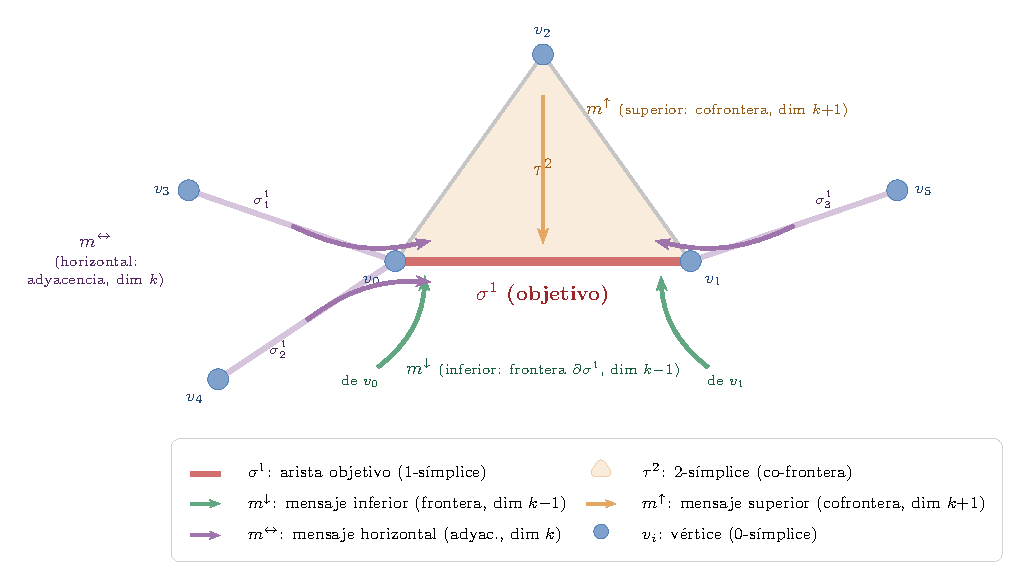
\includegraphics[width=0.8\textwidth]{images/simplicial_messages.pdf}
\caption{Three types of messages in Simplicial Attention Networks. A target edge (red) receives: \emph{lower} messages from its boundary vertices (green), \emph{upper} messages from triangles of which it is a face (orange), and \emph{horizontal} messages from adjacent edges (purple).}
\label{fig:simplicial_messages}
\end{figure}

\begin{definition}[Simplicial Message]\label{def:mensaje_simplicial}
For a $k$-simplex $\sigma$, we define different types of messages:

\textbf{Lower Message}: From incident $(k-1)$-simplices:
\begin{equation}
    \mathbf{m}_{\sigma}^{\text{lower}} = \sum_{\tau \in \partial_k(\sigma)} \alpha_{\tau \to \sigma} \mathbf{W}^{\text{lower}} \mathbf{h}_{\tau}
\end{equation}

\textbf{Upper Message}: From incident $(k+1)$-simplices:
\begin{equation}
    \mathbf{m}_{\sigma}^{\text{upper}} = \sum_{\rho: \sigma \in \partial_{k+1}(\rho)} \alpha_{\rho \to \sigma} \mathbf{W}^{\text{upper}} \mathbf{h}_{\rho}
\end{equation}

\textbf{Horizontal Message}: From adjacent $k$-simplices:
\begin{equation}
    \mathbf{m}_{\sigma}^{\text{horizontal}} = \sum_{\tau \in \mathcal{N}_k(\sigma)} \alpha_{\tau \to \sigma} \mathbf{W}^{\text{horizontal}} \mathbf{h}_{\tau}
\end{equation}
\end{definition}

\begin{definition}[Simplicial Attention Weights]\label{def:pesos_atencion_simplicial}
The attention weights incorporate orientation information:
\begin{align}
    \alpha_{\tau \to \sigma} &= \frac{\exp(\text{LeakyReLU}(\mathbf{a}^T [\mathbf{h}_{\tau} \| \mathbf{h}_{\sigma} \| \mathbf{e}_{\text{orient}}(\tau,\sigma)]))}{\sum_{\rho} \exp(\text{LeakyReLU}(\mathbf{a}^T [\mathbf{h}_{\rho} \| \mathbf{h}_{\sigma} \| \mathbf{e}_{\text{orient}}(\rho,\sigma)]))}
\end{align}
where $\mathbf{e}_{\text{orient}}(\tau,\sigma)$ encodes the orientation relation between simplices.
\end{definition}

\begin{definition}[Complete Simplicial Update]\label{def:actualizacion_simplicial}
The update of a $k$-simplex integrates all message types:
\begin{align}
    \mathbf{h}_{\sigma}^{(l+1)} = \sigma\left(\mathbf{W}^{\text{self}} \mathbf{h}_{\sigma}^{(l)} + \mathbf{m}_{\sigma}^{\text{lower}} + \mathbf{m}_{\sigma}^{\text{upper}} + \mathbf{m}_{\sigma}^{\text{horizontal}}\right)
\end{align}
\end{definition}

\subsubsection{Preservation of Topological Structure}

\begin{theorem}[Simplicial Equivariance]\label{thm:equivarianza_simplicial}
Simplicial Attention Networks are equivariant under automorphisms of simplicial complexes. If $\phi: \mathcal{K} \to \mathcal{K}$ is a simplicial automorphism, then:
\begin{equation}
    \text{SAN}(\phi(\mathbf{X})) = \phi(\text{SAN}(\mathbf{X}))
\end{equation}
\end{theorem}

\begin{proof}
A simplicial automorphism $\phi$ induces a permutation $P_k$ on the set of $k$-simplices that preserves the incidence relations: $\mathbf{B}_k P_{k-1} = P_k \mathbf{B}_k$. The simplicial update (\autoref{def:actualizacion_simplicial}) depends on the boundary matrices through the Laplacians $\mathbf{L}_k^{\text{up}}$ and $\mathbf{L}_k^{\text{down}}$. Since $P_k \mathbf{L}_k P_k^T = \mathbf{L}_k$ (the Laplacians commute with simplicial automorphisms), and the attention weights $\alpha_{\sigma\tau}$ depend on the representations through functions symmetric with respect to $\phi$, it follows that $P_k \cdot \text{SAN}(\mathbf{X}) = \text{SAN}(P_k \cdot \mathbf{X})$ for each dimension $k$.
\end{proof}

\begin{remark}[Chain Structure in SANs]\label{rem:respeto_estructura_cadenas}
For the linear component of a SAN (without nonlinear activation functions), the chain map property
\begin{equation}
    \text{SAN}_{\text{lin}}(\partial_k \mathbf{c}) = \partial_k \text{SAN}_{\text{lin}}(\mathbf{c})
\end{equation}
holds if the linear layer commutes with the boundary operator $\partial_k$. However, this property is generally false for the full network with nonlinear activation functions: element-wise nonlinearities violate the chain map condition. In practice, SAN architectures are designed to approximately preserve the topological structure (processing signals of each simplicial grade separately and respecting adjacencies), but exact commutativity with $\partial_k$ is not guaranteed.
\end{remark}

\begin{remark}[Approximate Homology Preservation]\label{cor:preservacion_homologia}
If a network were an exact chain map (that is, if it commuted with $\partial_k$), then it would induce a well-defined map on homology: cycles would map to cycles and boundaries to boundaries. Real SANs, by incorporating nonlinearities, only preserve the homological structure approximately. The ``Hodge-aware'' design of these architectures (which processes the components of the Hodge decomposition separately) seeks to maintain this property as far as possible.
\end{remark}

\subsection{Hodge Laplacian Attention}

\subsubsection{Motivation from Differential Geometry}

On differentiable manifolds, the Hodge Laplacian $\Delta = d \delta + \delta d$ (where $d$ is the exterior derivative and $\delta$ its adjoint) plays a central role in the theory of differential forms. Its discrete analog provides a powerful tool for the analysis of signals on simplicial complexes.

\begin{definition}[Discrete Hodge Laplacian]\label{def:hodge_laplacian_discreto}
For a simplicial complex $\mathcal{K}$ with an inner product, the Hodge Laplacian of order $k$ is:
\begin{align}
    \mathbf{L}_k &= \mathbf{B}_{k+1} \mathbf{B}_{k+1}^T + \mathbf{B}_k^T \mathbf{B}_k \\
    &= \mathbf{L}_k^{\text{up}} + \mathbf{L}_k^{\text{down}}
\end{align}
where $\mathbf{B}_k$ is the boundary matrix of the complex.
\end{definition}

\begin{theorem}[Spectral Decomposition of the Hodge Laplacian]\label{thm:descomposicion_hodge_laplacian}
The Hodge Laplacian admits the decomposition:
\begin{equation}
    \mathbf{L}_k = \mathbf{U}_k \boldsymbol{\Lambda}_k \mathbf{U}_k^T
\end{equation}
where $\boldsymbol{\Lambda}_k = \text{diag}(\lambda_1, \lambda_2, \ldots, \lambda_{n_k})$ with $0 = \lambda_1 \leq \lambda_2 \leq \cdots \leq \lambda_{n_k}$.
\end{theorem}

\begin{proof}
The Hodge Laplacian $\mathbf{L}_k = \mathbf{B}_{k+1}\mathbf{B}_{k+1}^T + \mathbf{B}_k^T\mathbf{B}_k$ is symmetric and positive semidefinite: for any vector $\mathbf{x}$, $\mathbf{x}^T \mathbf{L}_k \mathbf{x} = \|\mathbf{B}_{k+1}^T \mathbf{x}\|^2 + \|\mathbf{B}_k \mathbf{x}\|^2 \geq 0$. By the spectral theorem for real symmetric matrices, $\mathbf{L}_k$ admits an orthonormal basis of eigenvectors with nonnegative real eigenvalues. The multiplicity of $\lambda = 0$ is $\dim(\ker(\mathbf{L}_k)) = \beta_k$, the $k$-th Betti number.
\end{proof}

\textbf{Interpretation of the Eigenvalues.}\label{rem:interpretacion_autovalores_hodge}
\begin{itemize}
    \item $\lambda_1 = 0$ with multiplicity $\beta_k$ (Betti number)
    \item The eigenvectors corresponding to $\lambda_1$ are the harmonic forms
    \item Larger eigenvalues correspond to signals with greater ``curvature''
\end{itemize}

\subsubsection{Hodge Laplacian Attention Networks}

\begin{definition}[Hodge Spectral Filter]\label{def:filtro_espectral_hodge}
A spectral filter on the simplicial complex is defined as:
\begin{equation}
    \mathbf{g}_{\theta}(\mathbf{L}_k) = \sum_{i=0}^{K-1} \theta_i \mathbf{T}_i(\tilde{\mathbf{L}}_k)
\end{equation}
where $\mathbf{T}_i$ are Chebyshev polynomials and $\tilde{\mathbf{L}}_k = \frac{2\mathbf{L}_k}{\lambda_{\max}} - \mathbf{I}$.
\end{definition}

\begin{definition}[Hodge Laplacian Attention]\label{def:hodge_laplacian_attention}
Hodge Laplacian-based attention incorporates spectral information:
\begin{align}
    \mathbf{Q}_k &= \mathbf{g}_{\theta}^Q(\mathbf{L}_k) \mathbf{H}_k \mathbf{W}^Q \\
    \mathbf{K}_k &= \mathbf{g}_{\theta}^K(\mathbf{L}_k) \mathbf{H}_k \mathbf{W}^K \\
    \mathbf{V}_k &= \mathbf{g}_{\theta}^V(\mathbf{L}_k) \mathbf{H}_k \mathbf{W}^V
\end{align}

The attention mechanism is defined as:
\begin{equation}
    \text{HodgeAttention}(\mathbf{H}_k) = \text{softmax}\left(\frac{\mathbf{Q}_k \mathbf{K}_k^T}{\sqrt{d_k}}\right) \mathbf{V}_k
\end{equation}
\end{definition}

\begin{theorem}[Frequency Interpretation of Hodge Attention]\label{thm:interpretacion_frecuencial_hodge}
Hodge Laplacian Attention acts as a filter in the spectral domain of the simplicial complex:
\begin{equation}
    \widehat{\text{HodgeAttention}}(\lambda) = g_{\theta}^Q(\lambda) g_{\theta}^K(\lambda) \hat{\mathbf{h}}(\lambda)
\end{equation}
where $\hat{\mathbf{h}}(\lambda)$ is the spectral transform of the features.
\end{theorem}

\begin{proof}
Projecting onto the eigenvector basis $\{\mathbf{u}_i\}$ of the Hodge Laplacian (\autoref{thm:descomposicion_hodge_laplacian}), the spectral filters act diagonally: $g_\theta(\mathbf{L}_k) = \mathbf{U}_k g_\theta(\boldsymbol{\Lambda}_k) \mathbf{U}_k^T$. Then $\mathbf{Q}_k = g_\theta^Q(\mathbf{L}_k) \mathbf{H}_k \mathbf{W}^Q$ has spectral transform $\hat{\mathbf{Q}}_k(\lambda_i) = g_\theta^Q(\lambda_i) \hat{\mathbf{H}}_k(\lambda_i) \mathbf{W}^Q$, and analogously for $\mathbf{K}_k$. The attention score in the spectral domain is $\hat{\mathbf{Q}}_k^T \hat{\mathbf{K}}_k(\lambda_i) \propto g_\theta^Q(\lambda_i) g_\theta^K(\lambda_i)$, which modulates the original signal $\hat{\mathbf{h}}(\lambda_i)$. The full mechanism acts as a band-pass filter whose transfer function is the product of the Q and K filters.
\end{proof}

\paragraph{Topological Spectral Attention}

The eigenvalues of the Hodge Laplacian (\autoref{thm:descomposicion_hodge_laplacian}) provide spectral features that capture topological properties. Topological spectral attention incorporates these features via a learnable spectral bias:

\begin{equation}
\operatorname{SpectralAttn}_k = \operatorname{softmax}\left(\frac{\mathbf{Q}_k \mathbf{K}_k^T}{\sqrt{d_k}} + \mathbf{W}_{\lambda} \operatorname{diag}(\boldsymbol{\lambda}^{(k)})\right) \mathbf{V}_k
\label{eq:spectral_topological_attention}
\end{equation}

\paragraph{Filtering in Hodge Components}

The Hodge decomposition allows filtering information by separating the signals into exact, harmonic, and co-exact components:

\begin{align}
\mathbf{H}_{\text{exact}} &= \mathbf{P}_{\operatorname{Im}(\delta_{k-1})} \mathbf{H} \label{eq:exact_component} \\
\mathbf{H}_{\text{harmonic}} &= \mathbf{P}_{\operatorname{Ker}(\mathcal{L}_k)} \mathbf{H} \\
\mathbf{H}_{\text{coexact}} &= \mathbf{P}_{\operatorname{Im}(\delta_k^*)} \mathbf{H}
\end{align}
where $\mathbf{P}$ denotes orthogonal projections onto each subspace.

\subsection{Applications in Network and Complex Graph Analysis}

\subsubsection{Topological Data Analysis (TDA)}

\begin{definition}[TDA Pipeline for Deep Learning]\label{def:pipeline_tda_dl}
The integrated TDA-Deep Learning pipeline consists of:
\begin{enumerate}
    \item \textbf{Complex construction}: From data, construct $\mathcal{K}$ (Vietoris-Rips, Alpha, etc.)
    \item \textbf{Persistence computation}: Obtain diagrams $\text{Pers}_k(\mathcal{K})$
    \item \textbf{Vectorization}: Convert diagrams to vector representations
    \item \textbf{Learning}: Use as features for attention models
\end{enumerate}
\end{definition}

\begin{definition}[Vector Representations of Persistence]\label{def:representaciones_persistencia}
Common methods include:

\textbf{Persistence Images} \citep{adams2017persistence}:
\begin{equation}
    \rho_{\sigma,u}(x,y) = \sum_{(b,d) \in \text{Dgm}} \omega(b,d) \cdot \frac{1}{\sigma\sqrt{2\pi}} \exp\left(-\frac{(x-b)^2 + (y-(d-b))^2}{2\sigma^2}\right)
\end{equation}

\textbf{Persistence Landscapes}:
\begin{equation}
    \lambda_k(t) = k\text{-th largest value of } \min(t-b, d-t)
\end{equation}
for points $(b,d)$ in the diagram.
\end{definition}

\begin{algorithm}
\caption{Simplicial Attention with TDA}\label{alg:sat_tda}
\textbf{Input}: Dataset $\mathcal{X}$, filtration parameters $\epsilon_1 < \epsilon_2 < \cdots < \epsilon_m$

\begin{enumerate}
    \item \textbf{Build filtration}:
    \begin{align}
        K_i &= \text{VietorisRips}(\mathcal{X}, \epsilon_i) \quad \forall i
    \end{align}

    \item \textbf{Compute persistent homology}:
    \begin{align}
        \text{Dgm}_k &= \text{PersistentHomology}(K_0 \subseteq K_1 \subseteq \cdots \subseteq K_m)
    \end{align}

    \item \textbf{Generate topological features}:
    \begin{align}
        \mathbf{f}_{\text{topo}} &= \text{PersistenceImage}(\text{Dgm}_k)
    \end{align}

    \item \textbf{Apply Simplicial Attention}:
    \begin{align}
        \mathbf{h}^{(l+1)} &= \text{SAN}([\mathbf{h}^{(l)} \| \mathbf{f}_{\text{topo}}])
    \end{align}
\end{enumerate}

\textbf{Output}: Topologically enriched representations
\end{algorithm}

\subsubsection{Specific Applications}

\begin{application}[Brain Network Analysis]\label{app:redes_cerebrales}
In connectomics, brain data are modeled as simplicial complexes where:
\begin{itemize}
    \item \textbf{Vertices}: Brain regions (ROIs)
    \item \textbf{Edges}: Pairwise functional connections
    \item \textbf{Triangles}: Order-3 functional interactions
    \item \textbf{k-simplices}: Higher-order activation patterns
\end{itemize}

Hodge Laplacian Attention allows detecting anomalous patterns in:
\begin{align}
    \mathbf{A}_{\text{brain}} &= \text{HodgeAttention}(\mathbf{H}_{\text{roi}}, \mathbf{L}_{\text{connectome}})
\end{align}
\end{application}

\begin{application}[Social Network Analysis]\label{app:redes_sociales}
To detect communities and hierarchical structures:
\begin{enumerate}
    \item Build the clique complex of the social graph
    \item Apply a filtration by connection strength
    \item Use persistence to identify stable communities
    \item Apply Simplicial Attention for user classification
\end{enumerate}
\end{application}

\begin{theorem}[Expressive Power of SANs vs GATs]\label{thm:poder_expresivo_sans}
For graphs with rich topological structure, Simplicial Attention Networks are strictly more expressive than traditional Graph Attention Networks:
\begin{equation}
    \exists G: \quad \text{SAN}(G) \not\in \text{span}\{\text{GAT}(G'): G' \text{ is a graph}\}
\end{equation}
\end{theorem}

\begin{proof}
We construct a separating example. Consider two graphs $G_1$ and $G_2$ with the same 1-skeleton graph (same nodes and edges) but different higher-order simplicial complexes: $G_1$ contains a 2-simplex (filled triangle) $[v_1, v_2, v_3]$ and $G_2$ does not (it only has the three edges). Any \gls{GAT} operates exclusively on nodes and edges, so it produces the same output for $G_1$ and $G_2$ (since the 1-skeleton is identical). However, a SAN accesses the 2-simplices: the signal on the filled triangle of $G_1$ generates ``upper''-type messages (\autoref{def:actualizacion_simplicial}) that do not exist in $G_2$. In particular, $\beta_1(G_1) \neq \beta_1(G_2)$ (the filled triangle eliminates an independent cycle), and this topological difference is detectable by the harmonic components of the order-1 Hodge Laplacian.
\end{proof}

\begin{corollary}[Computational Advantage]\label{cor:ventaja_computacional_sans}
For problems with higher-order interactions, SANs require fewer parameters than equivalent multilayer \glspl{GAT}:
\begin{equation}
    |\theta_{\text{SAN}}| = O(d \cdot k_{\max}) \ll |\theta_{\text{GAT-equiv}}| = O(d \cdot L^2)
\end{equation}
where $k_{\max}$ is the maximum dimension of simplices and $L$ is the depth of the \gls{GAT}.
\end{corollary}

\begin{proof}
A SAN directly processes $k$-simplices for each dimension $k = 0, 1, \ldots, k_{\max}$, with $O(d)$ parameters per simplicial dimension (attention and feature transformation matrices). This gives a total of $O(d \cdot k_{\max})$ parameters.

A standard \gls{GAT} only operates on edges (1-simplices), so capturing order-$k$ interactions requires propagating information across $k$ hops. To capture interactions up to order $k_{\max}$, at least $L \geq k_{\max}$ layers are needed, each with $O(d \cdot L)$ parameters (the intermediate dimensions must grow with $L$ to avoid information loss). The total is $O(d \cdot L^2)$. Since SANs directly access higher-order interactions, they avoid the quadratic accumulation of parameters.
\end{proof}

\subsection{Connections with Diffusion Models and Differential Equations}

\subsubsection{Diffusion on Simplicial Complexes}

\begin{definition}[Simplicial Diffusion Equation]\label{def:ecuacion_difusion_simplicial}
The diffusion equation on a simplicial complex is written as:
\begin{equation}
    \frac{\partial \mathbf{f}_k}{\partial t} = -\mathbf{L}_k \mathbf{f}_k
\end{equation}
where $\mathbf{f}_k(t) \in \mathbb{R}^{n_k}$ represents signals on $k$-simplices.
\end{definition}

\begin{theorem}[Solution of the Diffusion Equation]\label{thm:solucion_difusion_simplicial}
The solution of the diffusion equation is:
\begin{equation}
    \mathbf{f}_k(t) = \exp(-t\mathbf{L}_k) \mathbf{f}_k(0) = \sum_{i=1}^{n_k} \exp(-t\lambda_i) \langle \mathbf{u}_i, \mathbf{f}_k(0) \rangle \mathbf{u}_i
\end{equation}
\end{theorem}

\begin{proof}
The equation $\dot{\mathbf{f}}_k = -\mathbf{L}_k \mathbf{f}_k$ is a linear system of ODEs with solution $\mathbf{f}_k(t) = \exp(-t\mathbf{L}_k) \mathbf{f}_k(0)$, where the matrix exponential is defined by its series $\exp(A) = \sum_{n=0}^\infty A^n/n!$. Using the spectral decomposition $\mathbf{L}_k = \mathbf{U}_k \boldsymbol{\Lambda}_k \mathbf{U}_k^T$ (\autoref{thm:descomposicion_hodge_laplacian}): $\exp(-t\mathbf{L}_k) = \mathbf{U}_k \exp(-t\boldsymbol{\Lambda}_k) \mathbf{U}_k^T = \mathbf{U}_k \operatorname{diag}(e^{-t\lambda_1}, \ldots, e^{-t\lambda_{n_k}}) \mathbf{U}_k^T$. Expanding $\mathbf{f}_k(0) = \sum_i \langle \mathbf{u}_i, \mathbf{f}_k(0)\rangle \mathbf{u}_i$, the result is obtained. The harmonic components ($\lambda_i = 0$) are stationary, while the high-frequency ones decay exponentially.
\end{proof}

\begin{definition}[Neural Diffusion on Complexes]\label{def:neural_diffusion_complejos}
A neural diffusion layer on simplicial complexes:
\begin{align}
    \mathbf{H}_k^{(l+1)} &= \sigma\left(\mathbf{W}^{(l)} \exp(-\alpha^{(l)} \mathbf{L}_k) \mathbf{H}_k^{(l)}\right)
\end{align}
where $\alpha^{(l)}$ controls the diffusion scale.
\end{definition}

This framework unifies concepts from differential geometry, algebraic topology, and deep learning, providing sophisticated mathematical tools for the analysis of data with complex topological structure.

The mathematical tools developed in the preceding sections (equivariant, spectral, hyperbolic, Clifford, and topological attention) find direct applications in molecular science, computational physics, and structural biology, where the preservation of symmetries such as $E(3)$, $SE(3)$, or the Lorentz group is essential for predicting physical properties. For an overview of these application domains, see the introduction (\autoref{ch:intro}).

\subsection[Transformers on CW Complexes]{\glspl{Transformer} on CW Complexes}

Cell complexes represent a natural generalization of graphs, allowing the capture of higher-order relations through cells of different dimensions \citep{bodnar2021cell}.

\paragraph{Multi-Dimensional Attention}

In a CW complex, attention must operate over multiple types of cells:

\begin{align}
\text{CWAttention}(\mathbf{X}) &= \bigoplus_{k=0}^{d} \text{Attention}^{(k)}(\mathbf{X}_k) \label{eq:cw_attention} \\
\text{Attention}^{(k)}(\mathbf{X}_k) &= \text{softmax}\left(\frac{\mathbf{Q}_k \mathbf{K}_k^T}{\sqrt{d_k}} + \mathbf{A}^{(k)}\right) \mathbf{V}_k
\end{align}

where $\mathbf{X}_k$ represents the features of $k$-cells and $\mathbf{A}^{(k)}$ is the adjacency matrix between $k$-cells.

\paragraph{Preservation of Incidence Relations}

The incidence relations between cells of different dimensions are preserved through:

\begin{equation}
\mathbf{M}^{(k,k-1)} = \text{IncidenceMatrix}(\text{Cell}_k, \text{Cell}_{k-1})
\label{eq:incidence_preservation}
\end{equation}

Inter-dimensional attention incorporates these relations:

\begin{equation}
\text{InterAttn}_{k \to k-1} = \text{softmax}(\mathbf{Q}_{k-1} (\mathbf{M}^{(k,k-1)} \mathbf{K}_k)^T) \mathbf{M}^{(k,k-1)} \mathbf{V}_k
\label{eq:inter_dimensional_attention}
\end{equation}

\subsection{Persistent Homology Attention}

Persistent homology provides a multiscale description of topological features, capturing how these evolve across spatial scales.

\paragraph{Persistence Diagrams}

For a filtration $X_0 \subseteq X_1 \subseteq \cdots \subseteq X_n$, the persistence diagrams record the birth and death time of topological features:

\begin{equation}
\text{Dgm}_k = \{(b_i, d_i) : H_k(X_{b_i}) \to H_k(X_{d_i}) \text{ is an isomorphism}\}
\label{eq:persistence_diagram}
\end{equation}

\paragraph{Integration into Attention}

The persistence diagrams are integrated into the attention mechanism through:

\begin{equation}
\alpha_{ij} = \text{softmax}\left(\frac{\mathbf{q}_i^T \mathbf{k}_j}{\sqrt{d}} + w \cdot \text{pers}(i,j)\right)
\label{eq:persistent_attention_weights}
\end{equation}

where $\text{pers}(i,j)$ encodes the topological persistence between points $i$ and $j$.

\paragraph{Persistence Functions}

The persistence function can take various forms:

\begin{align}
\text{pers}_{\text{lifetime}}(i,j) &= \sum_{(b,d) \in \text{Dgm}} (d-b) \cdot \mathbb{I}[\text{connected}(i,j,b,d)] \label{eq:lifetime_persistence} \\
\text{pers}_{\text{birth}}(i,j) &= \min\{b : (b,d) \in \text{Dgm}, \text{connected}(i,j,b,d)\} \\
\text{pers}_{\text{stability}}(i,j) &= \max_{(b,d) \in \text{Dgm}} (d-b) \cdot \mathbb{I}[\text{connected}(i,j,b,d)]
\end{align}

\paragraph{Advantages of Persistence}

The incorporation of persistent homology offers:

\begin{enumerate}
    \item \textbf{Robustness to noise}: Persistent features are more stable
    \item \textbf{Multiscale detection}: Captures patterns at multiple resolutions
    \item \textbf{Topological invariance}: Resistance to continuous deformations
    \item \textbf{Interpretability}: Direct connection with known geometric properties
\end{enumerate}

\subsection{Applications of Topological Algebra}

This advanced formulation finds applications in:

\begin{itemize}
    \item \textbf{Analysis of flows in networks}: Separation of irrotational and solenoidal components using Hodge
    \item \textbf{Electromagnetic processing}: Electric and magnetic fields as differential forms
    \item \textbf{Computational topology}: Analysis of cavities and holes in complex data
    \item \textbf{Time series analysis}: Capture of recurrent topological patterns with persistence
    \item \textbf{Anomaly detection}: Identification of unexpected topological changes
    \item \textbf{Dynamical systems}: Characterization of attractors and orbits through topology
\end{itemize}


\subsection{Outstanding Theoretical and Practical Challenges}

Despite significant advances, geometric attention mechanisms face fundamental challenges that require ongoing research.

\subsubsection{Limitations of Expressivity vs Efficiency}

\paragraph{The Complexity Dilemma}

The trade-off between expressivity and computational efficiency remains one of the central challenges. While traditional attention achieves $O(n^2)$ complexity, geometric approaches frequently increase the complexity due to:

\begin{enumerate}
    \item \textbf{Operations on Lie groups}: The cost of projections and lifting to high-dimensional spaces
    \item \textbf{Spectral analysis}: Eigendecomposition of Laplacians on large graphs
    \item \textbf{Parallel transport}: Geodesic computations on complex manifolds
    \item \textbf{Tensor products}: Dimensional expansion in irreducible representations
\end{enumerate}

\begin{definition}[Geometric Complexity Index]
For a geometric attention architecture with symmetry $G$, we define:
\begin{equation}
\text{ICG}(G, n) = \frac{\text{Cost}(G\text{-equivariance})}{\text{Cost}(\text{standard attention})} \cdot \frac{|\text{Orbit}(G)|}{n}
\label{eq:geometric_complexity_index}
\end{equation}
where $|\text{Orbit}(G)|$ measures the size of the orbits under the group action.
\end{definition}

\paragraph{Approximations and Trade-offs}

Recent developments in sub-quadratic architectures suggest that it is possible to preserve essential geometric properties with linear complexity:

\begin{remark}[Asymptotic Preservation of Equivariance]
Under certain regularity conditions, it is conjectured that linear-complexity models can approximate equivariant architectures with bounded error:
\begin{equation}
\|f_{\text{linear}}(g \cdot x) - g \cdot f_{\text{quadratic}}(x)\| \leq \epsilon_{\text{precision}}
\label{eq:linear_equivariance_approximation}
\end{equation}
The rigorous formalization of this bound and the precise conditions under which it holds remain an open problem.
\end{remark}

\subsubsection{Scalability to Massive Data}

\paragraph{Memory Limitations}

Modern foundation models require the processing of:
\begin{itemize}
    \item \textbf{Protein structures}: $>10^6$ atoms per macromolecular complex
    \item \textbf{Molecular simulations}: $10^9$ particles in temporally extended dynamics
    \item \textbf{Social network graphs}: $10^{12}$ connections in global platforms
    \item \textbf{LiDAR point clouds}: $10^8$ points per city scan
\end{itemize}

The required GPU memory scales as:

\begin{equation}
\text{Memory}_{\text{GDL}} = O(n^2 \cdot d_{\text{model}} \cdot |\text{Rep}(G)| \cdot \text{Precision})
\label{eq:gdl_memory_scaling}
\end{equation}

where $|\text{Rep}(G)|$ represents the dimension of the group representations.

\paragraph{Distribution Strategies}

Emerging solutions include:

\begin{enumerate}
    \item \textbf{Distributed Ring Attention}: Ring parallelization with communication overlapping
    \item \textbf{Geometric gradient checkpointing}: Selective recompute of expensive equivariant operations
    \item \textbf{Symmetry-aware quantization}: Preservation of equivariance under reduced precision
    \item \textbf{Structured sparsification}: Pruning that respects the group structure
\end{enumerate}

\subsubsection{Interpretability of Geometric Attention}

\paragraph{Visualization Complexity}

The interpretability of geometric attention mechanisms presents unique challenges:

\begin{itemize}
    \item \textbf{High-dimensional spaces}: Visualization of representations in $SO(3)$ or $SE(3)$
    \item \textbf{Multiple scales}: Attention operating simultaneously at various geometric resolutions
    \item \textbf{Non-linear interactions}: Tensor products and complex group operations
    \item \textbf{Temporal dependencies}: Evolution of attention patterns in dynamic sequences
\end{itemize}

\begin{definition}[Geometric Saliency]
For a $G$-equivariant attention mechanism, the saliency with respect to the group is defined as:
\begin{equation}
\text{Sal}_G(x_i, x_j) = \sum_{g \in G} w(g) \cdot \alpha_{ij}(g \cdot x_i, g \cdot x_j)
\label{eq:geometric_saliency}
\end{equation}
where $w(g)$ are weights associated with group elements.
\end{definition}

\paragraph{Analysis Tools}

The development of specialized tools includes:

\begin{enumerate}
    \item \textbf{Manifold projection}: Visualization of attention in interpretable 2D/3D spaces
    \item \textbf{Spectral analysis of patterns}: Decomposition of attention maps into frequency components
    \item \textbf{Symmetry traceability}: Tracking the preservation of equivariance across layers
    \item \textbf{Directed perturbation}: Sensitivity analysis with respect to specific geometric transformations
\end{enumerate}

\subsubsection{Theoretical Generalization}

\paragraph{Universal Approximation Limits}

The universal approximation results for geometric attention require extension:

\begin{remark}[Group-Conditioned Universal Approximation]
Let $\mathcal{F}_G$ be the space of $G$-equivariant functions on a geometric domain $\mathcal{M}$. It is conjectured that a geometric attention network can uniformly approximate any $f \in \mathcal{F}_G$ under the following conditions:
\begin{enumerate}
    \item The action of $G$ on $\mathcal{M}$ is piecewise transitive
    \item The representations used generate all the necessary irreducible representations
    \item The attention mechanism respects the causal structure of the domain
\end{enumerate}
This result extends the universal approximation conjecture for equivariant functions (see \autoref{rem:aproximacion_universal_clifford}) and remains an open problem.
\end{remark}

\paragraph{Generalization Bounds}

The generalization capacity is limited by:

\begin{equation}
\text{Error}_{\text{gen}} \leq \text{Error}_{\text{emp}} + \sqrt{\frac{\text{Dim}(\text{Rep}(G)) \log N}{N}}
\label{eq:geometric_generalization_bound}
\end{equation}

where $\text{Dim}(\text{Rep}(G))$ is the effective dimension of the representation space.

\section{Connections with CNNs and Future Directions}\label{sec:cnn_attention_connections}

This chapter has developed geometric attention mechanisms from multiple mathematical perspectives: group theory, spectral analysis, differential geometry, geometric algebra, and algebraic topology. To complete the unifying theoretical framework of Geometric Deep Learning, this final section establishes the fundamental connections with the Geometric Convolutional Neural Networks developed in \autoref{ch:cnn}, demonstrating the conceptual convergence of both paradigms under shared mathematical principles.

\subsection{Unifying Theoretical Framework: Geometric Message Passing}\label{subsec:marco_teorico_unificador}

Resuming the synthesis of \autoref{ch:gdl} (Section~\ref{subsec:message_passing_unificador}) and connecting with the deep analysis of geometric CNNs, we establish the following unifying framework that subsumes both convolutions and attention under a common mathematical abstraction.

\begin{definition}[Generalized Geometric Message Passing]\label{def:message_passing_geometrico_generalizado}
Let $\mathcal{D}$ be a geometric domain (Euclidean grid, graph, manifold, homogeneous space), $G$ a group of symmetries, and $\mathcal{F}(\mathcal{D})$ the space of signals over $\mathcal{D}$. A Geometric Message Passing operator is a family of transformations:
\begin{equation}
    \mathcal{T}^{(G)}: \mathcal{F}(\mathcal{D}) \to \mathcal{F}(\mathcal{D})
    \label{eq:message_passing_geometrico_generalizado}
\end{equation}
that satisfies:
\begin{enumerate}
    \item \textbf{G-Equivariance}: $\mathcal{T}^{(G)}(g \cdot f) = g \cdot \mathcal{T}^{(G)}(f)$ for all $g \in G$
    \item \textbf{Geometric Locality}: Support determined by the geometry of $\mathcal{D}$
    \item \textbf{Compositionality}: $\mathcal{T}^{(G)}_2 \circ \mathcal{T}^{(G)}_1$ preserves geometric properties
\end{enumerate}
\end{definition}

\begin{theorem}[Fundamental CNN-Attention Correspondence]\label{thm:correspondencia_cnn_attention}
There exists a bijective correspondence between geometric convolutions and geometric attention mechanisms through Geometric Message Passing:
\begin{align}
    \text{\textbf{Geometric CNN}} &\leftrightarrow \text{Message Passing with fixed weights} \\
    \text{\textbf{Geometric Attention}} &\leftrightarrow \text{Message Passing with adaptive weights} \\
    \text{\textbf{Hybrid}} &\leftrightarrow \text{Message Passing with partial structure}
\end{align}
This correspondence preserves the properties of equivariance, expressive power, and computational complexity.
\end{theorem}

\begin{proof}[Proof sketch]
The proof is constructed by establishing formal equivalence at three levels:

\textbf{Algebraic Level}: Both operations are expressed as generalized convolutions in the group algebra $\mathbb{C}[G]$. For CNNs, the kernel is fixed: $k_g$; for attention, it is dynamic: $\alpha_{ij}(\mathbf{h}_i, \mathbf{h}_j)$.

\textbf{Spectral Level}: In the Fourier basis of the geometric domain, both operations correspond to multiplication by transfer functions. CNNs use fixed spectral filters $\hat{k}(\lambda)$; attention uses adaptive filters $\hat{\alpha}(\lambda; \mathbf{h})$.

\textbf{Geometric Level}: The neighborhood structure determines the support of integration. CNNs integrate over fixed neighborhoods; attention integrates with weights that depend on the content and respect the underlying geometry.
\end{proof}

\subsection{Table of Theoretical Equivalences}\label{subsec:tabla_equivalencias}

The following systematic analysis establishes the direct correspondences between fundamental concepts developed in both chapters:

\begin{table}[H]
\centering
\caption{Fundamental Mathematical Equivalences: CNNs $\leftrightarrow$ Attention}
\label{tab:cnn_attention_equivalencias_fundamentales}
\begin{tabular}{|p{4cm}|p{4cm}|p{6cm}|}
\hline
\textbf{Geometric CNN} & \textbf{Geometric Attention} & \textbf{Unifying Principle} \\
\hline\hline
\textit{Group Convolution} \\
(\autoref{sec:group_convolutions}) & \textit{G-Equivariant Attention} \\
(Section~\ref{subsec:equivariant_attention}) & Operations that commute with the group action $G$ \\
\hline
\textit{Spectral Filters} \\
$\hat{f}(\lambda_i) = g(\lambda_i) \hat{x}(\lambda_i)$ & \textit{Spectral Attention} \\
$A_{ij} = \text{softmax}(f(\lambda_i, \lambda_j))$ & Multiplication in the Fourier domain of the Laplacian \\
\hline
\textit{Gauge Convolution} \\
(\autoref{sec:gauge_cnns}) & \textit{Gauge-Equivariant Attention} & Respect for local coordinate transformations \\
\hline
\textit{Steerable CNNs} \\
$f \mapsto \rho(g) f$ & \textit{Steerable Attention} \\
$A \mapsto \rho(g) A \rho(g)^{-1}$ & Coherent action on vector fields \\
\hline
\textit{Spherical CNNs} \\
Spherical harmonics $Y_\ell^m$ & \textit{Spherical Attention} \\
Inner products in $L^2(S^2)$ & Harmonic analysis on the sphere \\
\hline
\textit{Manifold CNNs} \\
Parallel transport & \textit{Riemannian Attention} \\
Riemannian connections & Intrinsic geometry of manifolds \\
\hline
\textit{ChebNet} \\
Chebyshev polynomials & \textit{Polynomial Attention} \\
Polynomial approximation & Efficient spectral localization \\
\hline
\end{tabular}
\end{table}

\begin{remark}[Hierarchy of Architectural Generalization]\label{rem:jerarquia_generalizacion}
The architectures of Geometric Deep Learning form a natural hierarchy of generalization:
\begin{equation}
\text{ANN} \subset \text{CNN} \subset \text{G-CNN} \subset \text{Manifold-CNN} \stackrel{\text{dual}}{\leftrightarrow} \text{Attention} \subset \text{G-Attention} \subset \text{Manifold-Attention}
\end{equation}
where each inclusion preserves fundamental geometric properties while increasing expressivity.
\end{remark}

\subsection{Deep Comparative Analysis: Rigidity vs. Adaptability}\label{subsec:rigidez_adaptabilidad}

One of the most fundamental distinctions between convolutional and attention paradigms lies in the balance between imposed structure (rigidity) and learnable flexibility (adaptability). This tension can be formalized mathematically:

\begin{definition}[Rigidity-Adaptability Spectrum]\label{def:espectro_rigidez_adaptabilidad}
For a neural architecture $\mathcal{A}$ operating over a domain $\mathcal{D}$, we define:
\begin{align}
    \text{Rigidity}(\mathcal{A}) &= \frac{\dim(\text{Imposed symmetries})}{\dim(\text{Parameter space})} \\
    \text{Adaptability}(\mathcal{A}) &= \frac{\dim(\text{Content-dependent weights})}{\dim(\text{Parameter space})}
\end{align}
with the fundamental constraint: $\text{Rigidity}(\mathcal{A}) + \text{Adaptability}(\mathcal{A}) \leq 1$.
\end{definition}

\begin{remark}[Fundamental Rigidity-Adaptability Trade-off]\label{rem:tradeoff_rigidez_adaptabilidad}
For Geometric Deep Learning architectures there is a fundamental trade-off:
\begin{equation}
    \text{Theoretical Guarantees} \propto \text{Rigidity}(\mathcal{A})
\end{equation}
\begin{equation}
    \text{Expressive Capacity} \propto \text{Adaptability}(\mathcal{A})
\end{equation}
The optimal architectures maximize $\text{Rigidity} \times \text{Adaptability}$ subject to the constraints of the problem.
\end{remark}

\begin{example}[Analysis of the Spectrum]\label{ex:analisis_espectro}
Consider the progression:
\begin{align}
    \text{Classical CNN}: &\quad \text{Rigidity} = 0.9, \text{Adaptability} = 0.1 \\
    \text{Group CNN}: &\quad \text{Rigidity} = 0.7, \text{Adaptability} = 0.3 \\
    \text{Graph Attention}: &\quad \text{Rigidity} = 0.3, \text{Adaptability} = 0.7 \\
    \text{Full Transformer}: &\quad \text{Rigidity} = 0.1, \text{Adaptability} = 0.9
\end{align}
This explains why CNNs provide better generalization guarantees with less data, while Transformers require massive data but achieve greater expressivity.
\end{example}

\subsection{Convergence of Paradigms: Mathematical Analysis}\label{subsec:convergencia_paradigmas}

Recent developments (2023-2024) suggest a conceptual convergence between convolutional and attention paradigms. This convergence can be formalized mathematically:

\begin{conjecture}[CNN-Attention Convergence]\label{conj:convergencia_cnn_attention}
For sequences of architectures $\{\mathcal{C}_n\}$ (CNNs with increasing complexity) and $\{\mathcal{A}_n\}$ (Attention with increasing structure), there exists a common limit:
\begin{equation}
    \lim_{n \to \infty} d(\mathcal{C}_n, \mathcal{A}_n) = 0
\end{equation}
where $d$ is a metric on the space of functionals over $\mathcal{F}(\mathcal{D})$, and the convergence occurs in the topology of compact operators.
\end{conjecture}

\textbf{Heuristic evidence.} The conjecture is supported by three observations:

\textbf{1. Spectral approximation}: Both families of operators can be approximated arbitrarily well by finite-dimensional spectral operators.

\textbf{2. Density in function spaces}: The set of geometric convolutions is dense in the space of equivariant operators, and attention mechanisms with geometric constraints converge to the same limit set.

\textbf{3. Adaptive regularization}: Modern regularization techniques (geometric dropout, adaptive normalization) cause both families to converge toward the same optimal bias-variance regime.

\subsubsection{Convergence Architectures}

The architectures that exemplify this convergence include:

\begin{definition}[ConvNext-Attention Hybrid]\label{def:convnext_attention}
A hybrid architecture that combines:
\begin{itemize}
    \item \textbf{Convolutional kernel}: To process local features with geometric guarantees
    \item \textbf{Attention heads}: To capture adaptive global dependencies
    \item \textbf{Dynamic switching}: A learnable mechanism that decides when to use each component
\end{itemize}
\end{definition}

\begin{definition}[Geometric Retentive Networks]\label{def:retentive_networks_geometricas}
Extension of the retentive mechanism to geometric domains:
\begin{equation}
    \text{Retention}(Q, K, V) = Q \odot \sum_{j} \text{decay}(d_\mathcal{M}(i,j)) \cdot K_j \odot V_j
\end{equation}
where $d_\mathcal{M}$ is the geodesic distance in the geometric domain $\mathcal{M}$.
\end{definition}

\subsection{Future Theoretical Developments}\label{subsec:desarrollos_teoricos_futuros}

\subsubsection{Unified Expressivity Limits}

\begin{conjecture}[Universal Limits of Geometric Approximation]\label{conj:limites_universales}
For every continuous function $f: \mathcal{M} \to \mathbb{R}$ over a compact manifold $\mathcal{M}$, and every $\epsilon > 0$, there exist CNN and Attention architectures of complexities $C_{CNN}(\epsilon)$ and $C_{Att}(\epsilon)$ such that:
\begin{equation}
    \frac{C_{Att}(\epsilon)}{C_{CNN}(\epsilon)} \to 1 \quad \text{as } \epsilon \to 0
\end{equation}
This conjecture suggests that the difference in architectural complexity vanishes in the limit of perfect approximation.
\end{conjecture}

\subsubsection{Geometric Information Theory}

\begin{definition}[Geometric Fisher Entropy]\label{def:entropia_geometrica_fisher}
For a distribution $p$ over a Riemannian manifold $(\mathcal{M}, g)$, the geometric entropy is defined as:
\begin{equation}
    H_g(p) = -\int_\mathcal{M} p(x) \log p(x) \sqrt{\det g(x)} \, dx
\end{equation}
This quantity captures both the statistical uncertainty and the underlying geometric complexity.
\end{definition}

\begin{conjecture}[Principle of Minimal Geometric Information]\label{conj:principio_informacion_minima}
The optimal GDL architectures minimize the geometric information necessary to represent the target function:
\begin{equation}
    \mathcal{A}^* = \arg\min_\mathcal{A} \left[ \mathcal{L}(\mathcal{A}) + \lambda H_g(\text{representations}_\mathcal{A}) \right]
\end{equation}
where $\mathcal{L}$ is the empirical loss and $\lambda$ controls the information-precision trade-off.
\end{conjecture}

\subsubsection{Geometric Meta-Learning}

\begin{definition}[Geometric Meta-Learner]\label{def:meta_learner_geometrico}
A system that automatically learns the relevant symmetries of a domain:
\begin{equation}
    \text{Meta-GDL}: \mathcal{D} \mapsto G_{\text{optimal}} \mapsto \mathcal{A}_{G_{\text{optimal}}}
\end{equation}
where $\mathcal{D}$ is the data, $G_{\text{optimal}}$ is the discovered group of symmetries, and $\mathcal{A}_{G_{\text{optimal}}}$ is the resulting architecture.
\end{definition}

\subsection{Final Reflection: Toward a Unified Theory}\label{subsec:reflexion_final}

The analyses presented in this chapter and in \autoref{ch:cnn} converge toward a fundamental conclusion: the distinction between "convolutional" and "attention" is increasingly less relevant from a deep theoretical perspective. Both paradigms represent different points on a continuum of geometric operators that process structured information.

The future of Geometric Deep Learning does not lie in the competition between paradigms, but in their intelligent synthesis. The most powerful architectures will combine the stability and efficiency of geometric convolutions with the flexibility and expressivity of adaptive attention, guided by deep mathematical principles rather than ad hoc heuristics.

\begin{remark}[Principle of Architectural Synthesis]\label{rem:principio_sintesis}
For every geometric problem with known structure $\mathcal{S}$ and required adaptability $\mathcal{A}$, there exists an optimal hybrid architecture:
\begin{equation}
    \mathcal{H}^* = \arg\min_{\mathcal{H}} \left[ \mathcal{L}(\mathcal{H}) + \lambda_1 d(\mathcal{H}, \mathcal{S}) + \lambda_2 (1 - \text{Adaptability}(\mathcal{H})) \right]
\end{equation}
where $d(\mathcal{H}, \mathcal{S})$ measures the distance to the known structure and the parameters $\lambda_i$ balance the constraints.
\end{remark}

This synthesis represents more than a technical convergence: it symbolizes the maturation of the field toward unifying principles that transcend historical divisions. As we will demonstrate in the next experimental chapter, this theoretical unification translates into measurable practical advantages and opens new possibilities for addressing the great scientific and technological challenges of the 21st century.

Geometry, as has been the case throughout the history of mathematics and physics, once again provides the unifying language needed to understand and exploit the apparent complexity of modern machine learning systems. In this geometric synthesis lies not only the understanding of the present, but also the conceptual tools to build the future of deep learning.
